\section{Анализ требований к программному средству}
\label{sec:freq}
\subsection{Описание функциональности ПС}
Основываясь на требованиях изложенных в разделе \ref{sec:domain:requirements} и диаграмме вариантов использования, рисунок \ref{fig:freg:usecase}, разрабатываемое ПС должно выполнять следующие функции:

\begin{itemize}
	\item регистрация пользователя;
	\item авторизация пользователя;
	\item просмотр сохраненных образцов почерка;
	\item удаление сохраненных образцов почерка;
	\item добавление нового образца почерка;
	\item выделение признаков образца почерка;
	\item определение параметров личности;
	\item пакетное добавление образцов почерка;
	\item обновление образцов почерка.
\end{itemize}

\begin{figure}[ht]
\centering
    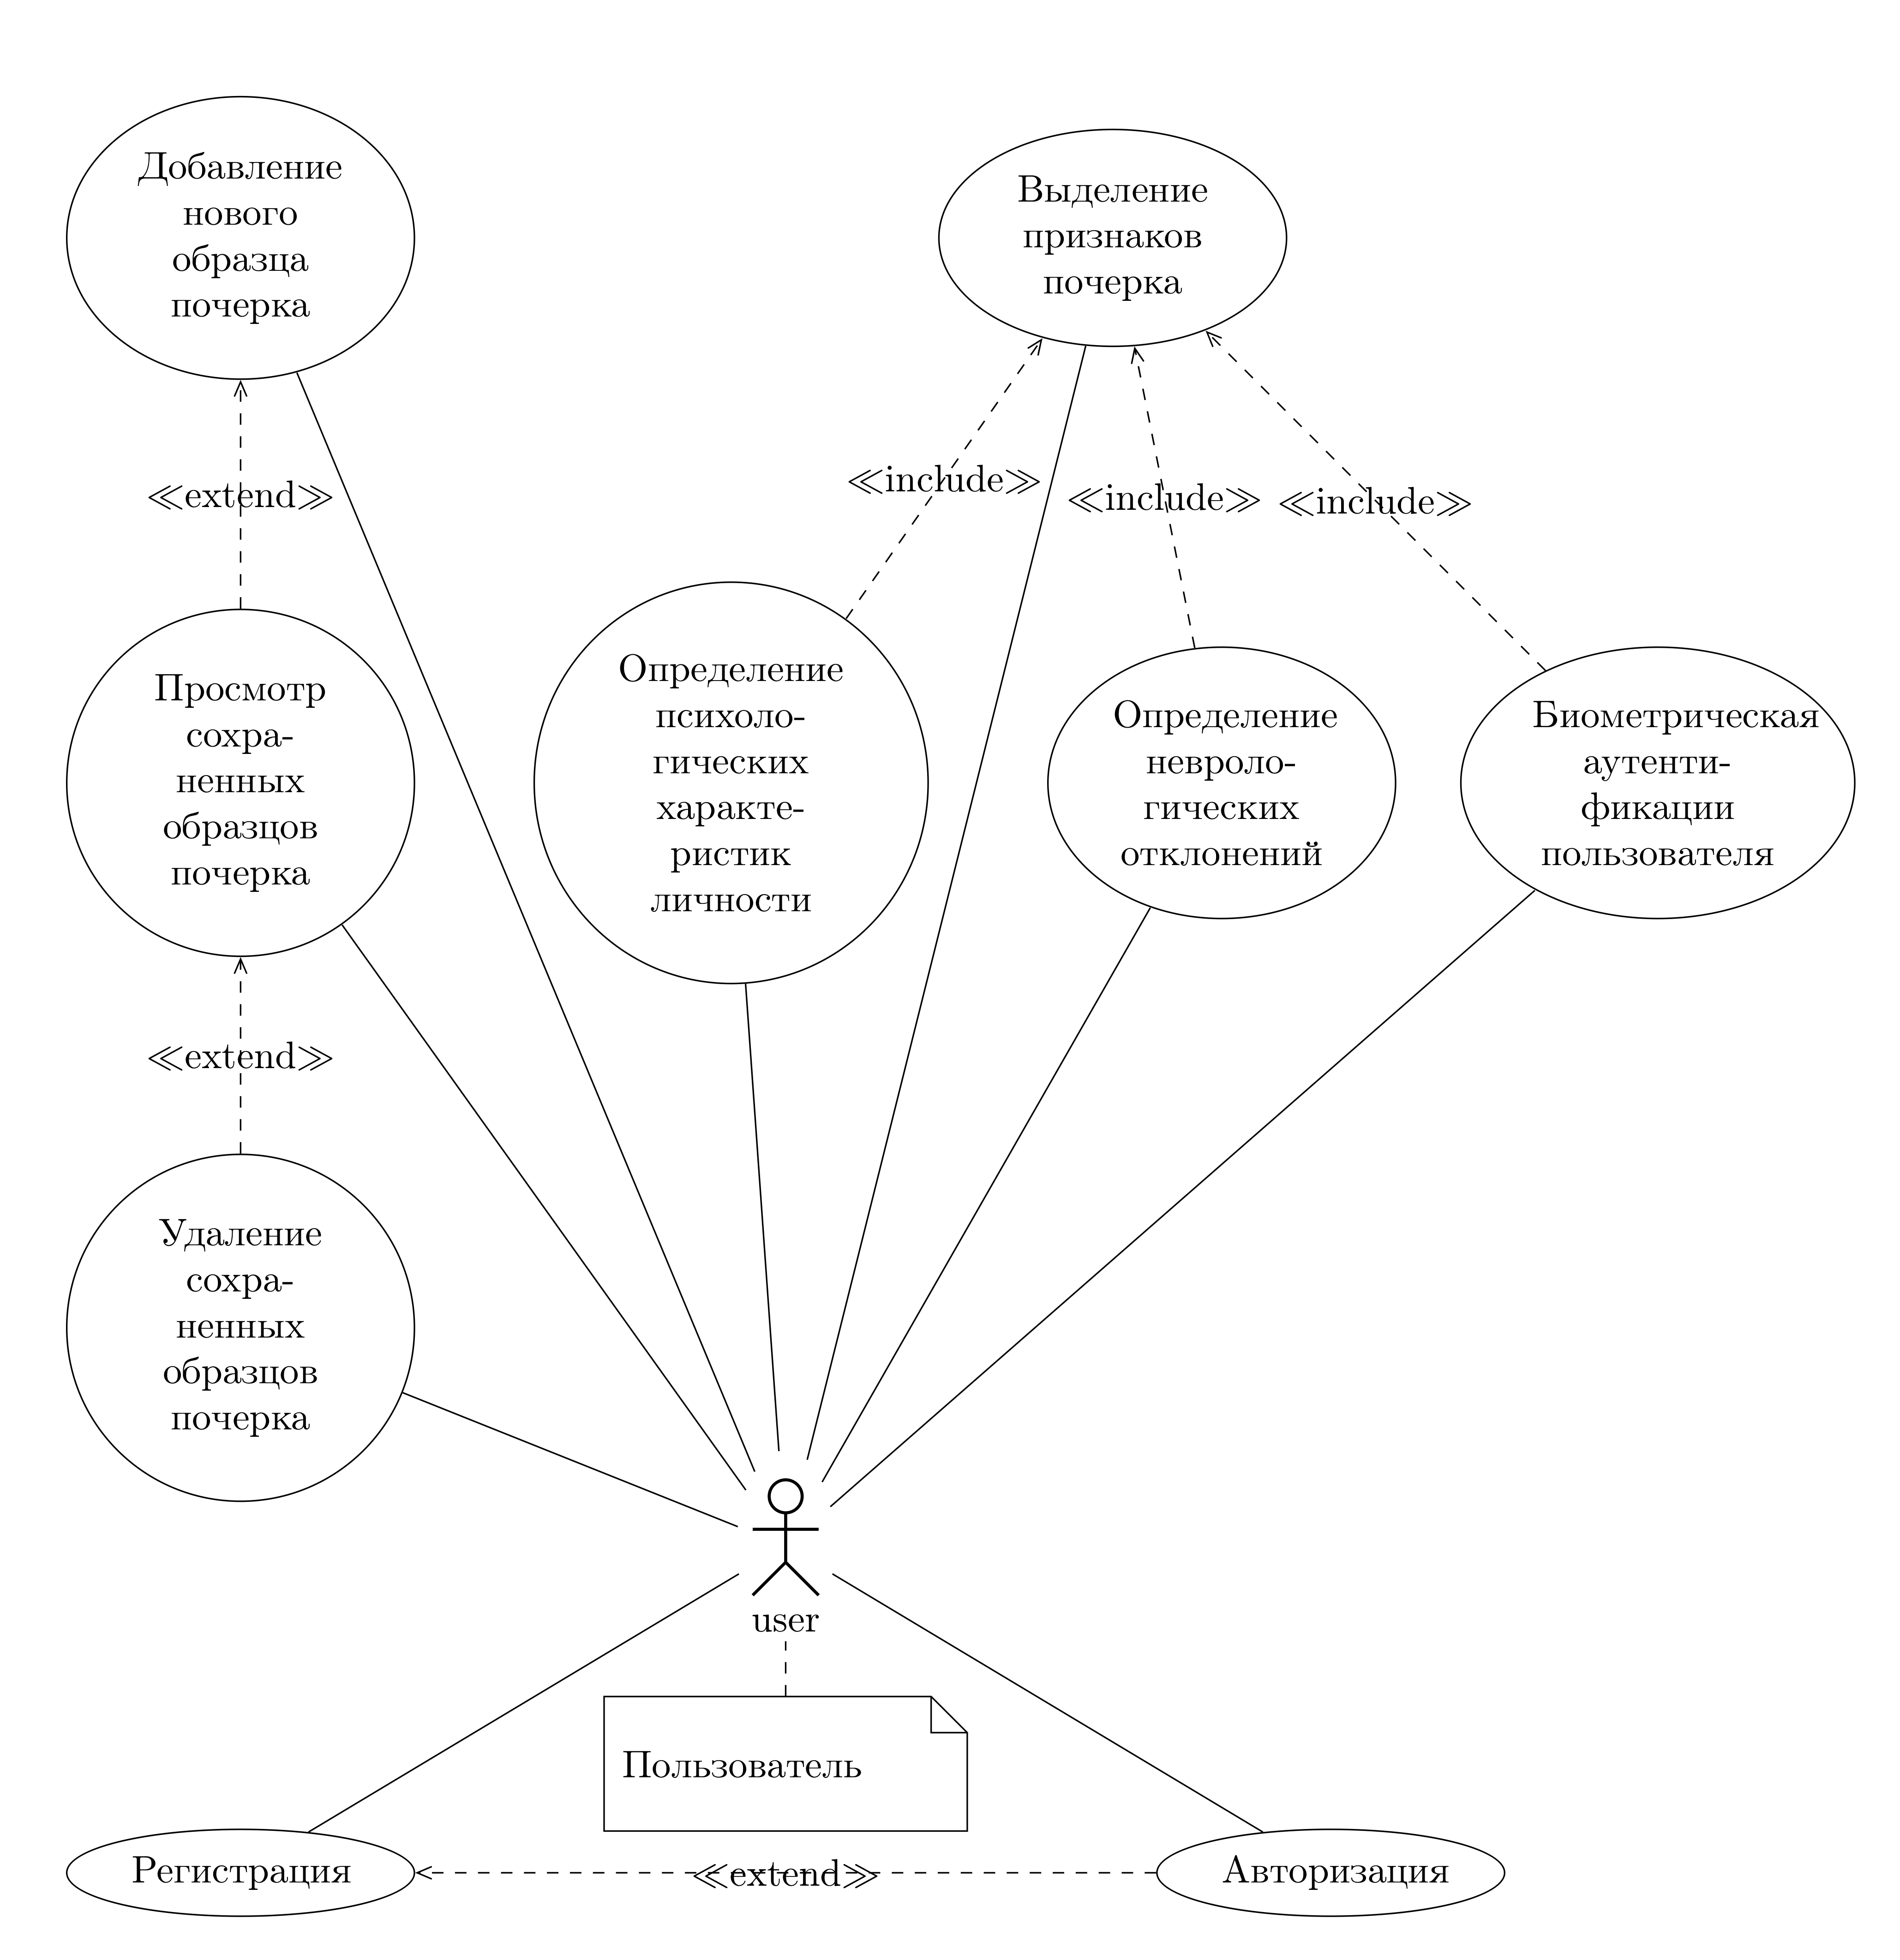
\includegraphics[scale=0.4]{figures/use_case.png}  
    \caption{Диаграмма вариантов использования}
  \label{fig:freg:usecase}
\end{figure}

Перечисленные функции позволят обеспечить полноценное функционирование программного средства, так как они покрываю все базовые операции хранения данных, а так же включают специализированные операции выделения признаков почерка и из классификации. Так же стоит отметить, что для полноценной промышленного использования программного средства необходимо соблюдение следующих требований:
\begin{itemize}
  \item независимая работа режимов выделения признаков рукописного текста и классификации;
  \item контроль сложности пароля;
  \item контроль размера образцов почерка;
  \item пароль не должен хранится в базе данных в открытов виде;
  \item контроль размера загружаемого образца почерка;
  \item асинхронное взаимодействие всех компонентов;
  \item параметры текста представляют собой вещественные значения с точностью до четырех знаков после запятой;
  \item использование JWT-маркеры для аутентификации и авторизации пользователей сервисами.
\end{itemize}

\subsection{Спецификация функциональных требований}
На основании функций программного средства разработана спецификация требований. 
\subsubsection{Регистрация пользователя}
\label{sec:freq:reg}
\begin{itemize}
	\item возможность регистрации должна быть доступна из пользовательского веб-интерфейса;
	\item пароль при регистрации должен проверяться на сложность(должен содержать не менее восьми символов в верхнем и нижнем регистрах и \mbox{цифры);}
	\item авторизационные данные пользователя должны передаваться по защищенному соединению.
\end{itemize}

\subsubsection{Авторизация пользователя}
\label{sec:freq:auth}
\begin{itemize}
	\item авторизационные данные пользователя должны передаваться по защищенному соединению;
	\item пароль пользователя не должен передаваться в явном виде (вычисления хеша в браузере);
 	\item сообщение об ошибке при вводе неверное логина или пароля не должно сообщать что именно введено неправильно.
\end{itemize}

\subsubsection{Просмотр сохраненных образцов почерка}
\label{sec:freq:show}
\begin{itemize}
	\item список ранее загруженных образцов доступен на главной странице пользователя;
	\item изображение и дополнительная информация(признаки почерка, параметры личности) должны загружаться только после выбора изображения из списка;
	\item пользователь имеет возможность запустить процесс выделения признаков почерка;
	\item пользователь имеет возможность запустить процесс определения параметров личности, если процесс выделения признаков почерка еще не был выполнен, то он будет запущен и по окончанию начнется процесс определения параметров личности.
\end{itemize}

\subsubsection{Удаление сохраненных образцов почерка}
\label{sec:freq:delete}
\begin{itemize}
	\item возможность удаления сохраненных образцов почерка должна быть доступна из пользовательского веб"=интерфейса страница просмотра образца;
	\item при удалении должно запрашиваться подтверждение действия пользователя с сообщением о последствиях;
	\item реальное удаление образца происходит через неделю после подтверждения удаления пользователем (возможность восстановить файл при ошибочном удалении).
\end{itemize}

\subsubsection{Добавление нового образца почерка}
\label{sec:freq:add}
\begin{itemize}
	\item возможность добавить новый образец доступна на главной странице пользователя;
	\item возможно добавить образцы в форматах jpg(jpeg), bmp и png;
	\item добавляемый образце должен иметь размер более 0 и менее 10 MB;
	\item после добавления нового образца пользователь переходит на страницу просмотра образца.
\end{itemize}

\subsubsection{Выделение признаков образца почерка}
\label{sec:freq:extract_features}
\begin{itemize}
	\item возможность выделение признаков образца почерка должна быть доступна из пользовательского веб-интерфейса страница просмотра образца;
	\item выделенные признаки образца почерка передаются по сети и хранятся в виде JSON-объекта;
	\item до завершения выделения признаков на странице отображается индикатор обработки в виде вращающегося круга.
\end{itemize}

\subsubsection{Определение параметров личности}
\label{sec:freq:psiho_analysis}
\begin{itemize}
	\item возможность определение параметров личности должна быть доступна из пользовательского веб-интерфейса страницы просмотра образца;
	\item определение параметров личности передаются по сети и хранятся в виде JSON-объекта;
	\item JSON-объект описывающий параметры личности содержит текстовое описание и метку класса;
	\item до завершения определения параметров личности на странице отображается индикатор отработки в виде вращающегося круга.
\end{itemize}

\subsubsection{Пакетное добавление образцов почерка}
\label{sec:freq:package_add}
\begin{itemize}
	\item возможность пакетного добавления новых образцов доступна на главной странице администратора;
	\item процессы выделения признаков и параметров личности начинаются автоматически;
	\item до завершения обработки изображений на странице отображается индикатор обработки в виде вращающегося круга.
\end{itemize}

\subsubsection{Обновление образцов почерка}
\label{sec:freq:update}
\begin{itemize}
	\item обновление образца происходит после выделение каждого признака;
	\item обновление образца происходит после классификации образца.
\end{itemize}

\subsubsection{Пользовательский интерфейс программного средства}
\begin{itemize}
	\item пользовательский интерфейс представляет собой Web-страницу;
	\item пользовательский интерфейс поддерживает русский и английский \mbox{языки;}
	\item возможность смены языка доступна пользователю на любой \mbox{странице;}
	\item поддержка Google Chrome и Firefox последних версий;
\end{itemize}

Поддержка операционных систем Windows, Linux, MacOS обеспечивается использованием <<тонкого клиента>> и ограничена только поддержкой данными системами версий браузеров.
Разрабатываемое программное средство не должно налагать ограничений на количество обрабатываемых и хранимых образцов почерка.